\documentclass{article}

% these packages let you do math
\usepackage{amsmath}
\usepackage{amssymb}

% we need these packages for fancy R tables
\usepackage{booktabs}
\usepackage{float}
\usepackage{colortbl}
\usepackage{xcolor}

% these packages play with the spacing/margins of the document. Uncomment the commands on lines 16 and 17 to see what they do.
\usepackage{a4wide}
\usepackage{setspace}
\usepackage{geometry}
\usepackage{parskip}
%\doublespacing
%\geometry{margin=1.5in}

% this package helps us with including images. Setting the graphics path makes it easier to refer to things in the \includegraphics command.
\usepackage{graphicx}
\graphicspath{ {../figures/} }

% make some hyperlinks using the \href command
\usepackage{hyperref}
\hypersetup{
    colorlinks=true,
    linkcolor=black,
    urlcolor=blue
}

% set the author, title, and date of the document. \maketitle adds it to the document.
\author{Adhi Rajaprabhakaran}
\title{Adhi's Paper on NLSY97 Incarceration Data}
\date{Spring 2022}

\begin{document}
\maketitle


\section{Incarceration Analysis}

\begin{figure}[H]
    \begin{center}
        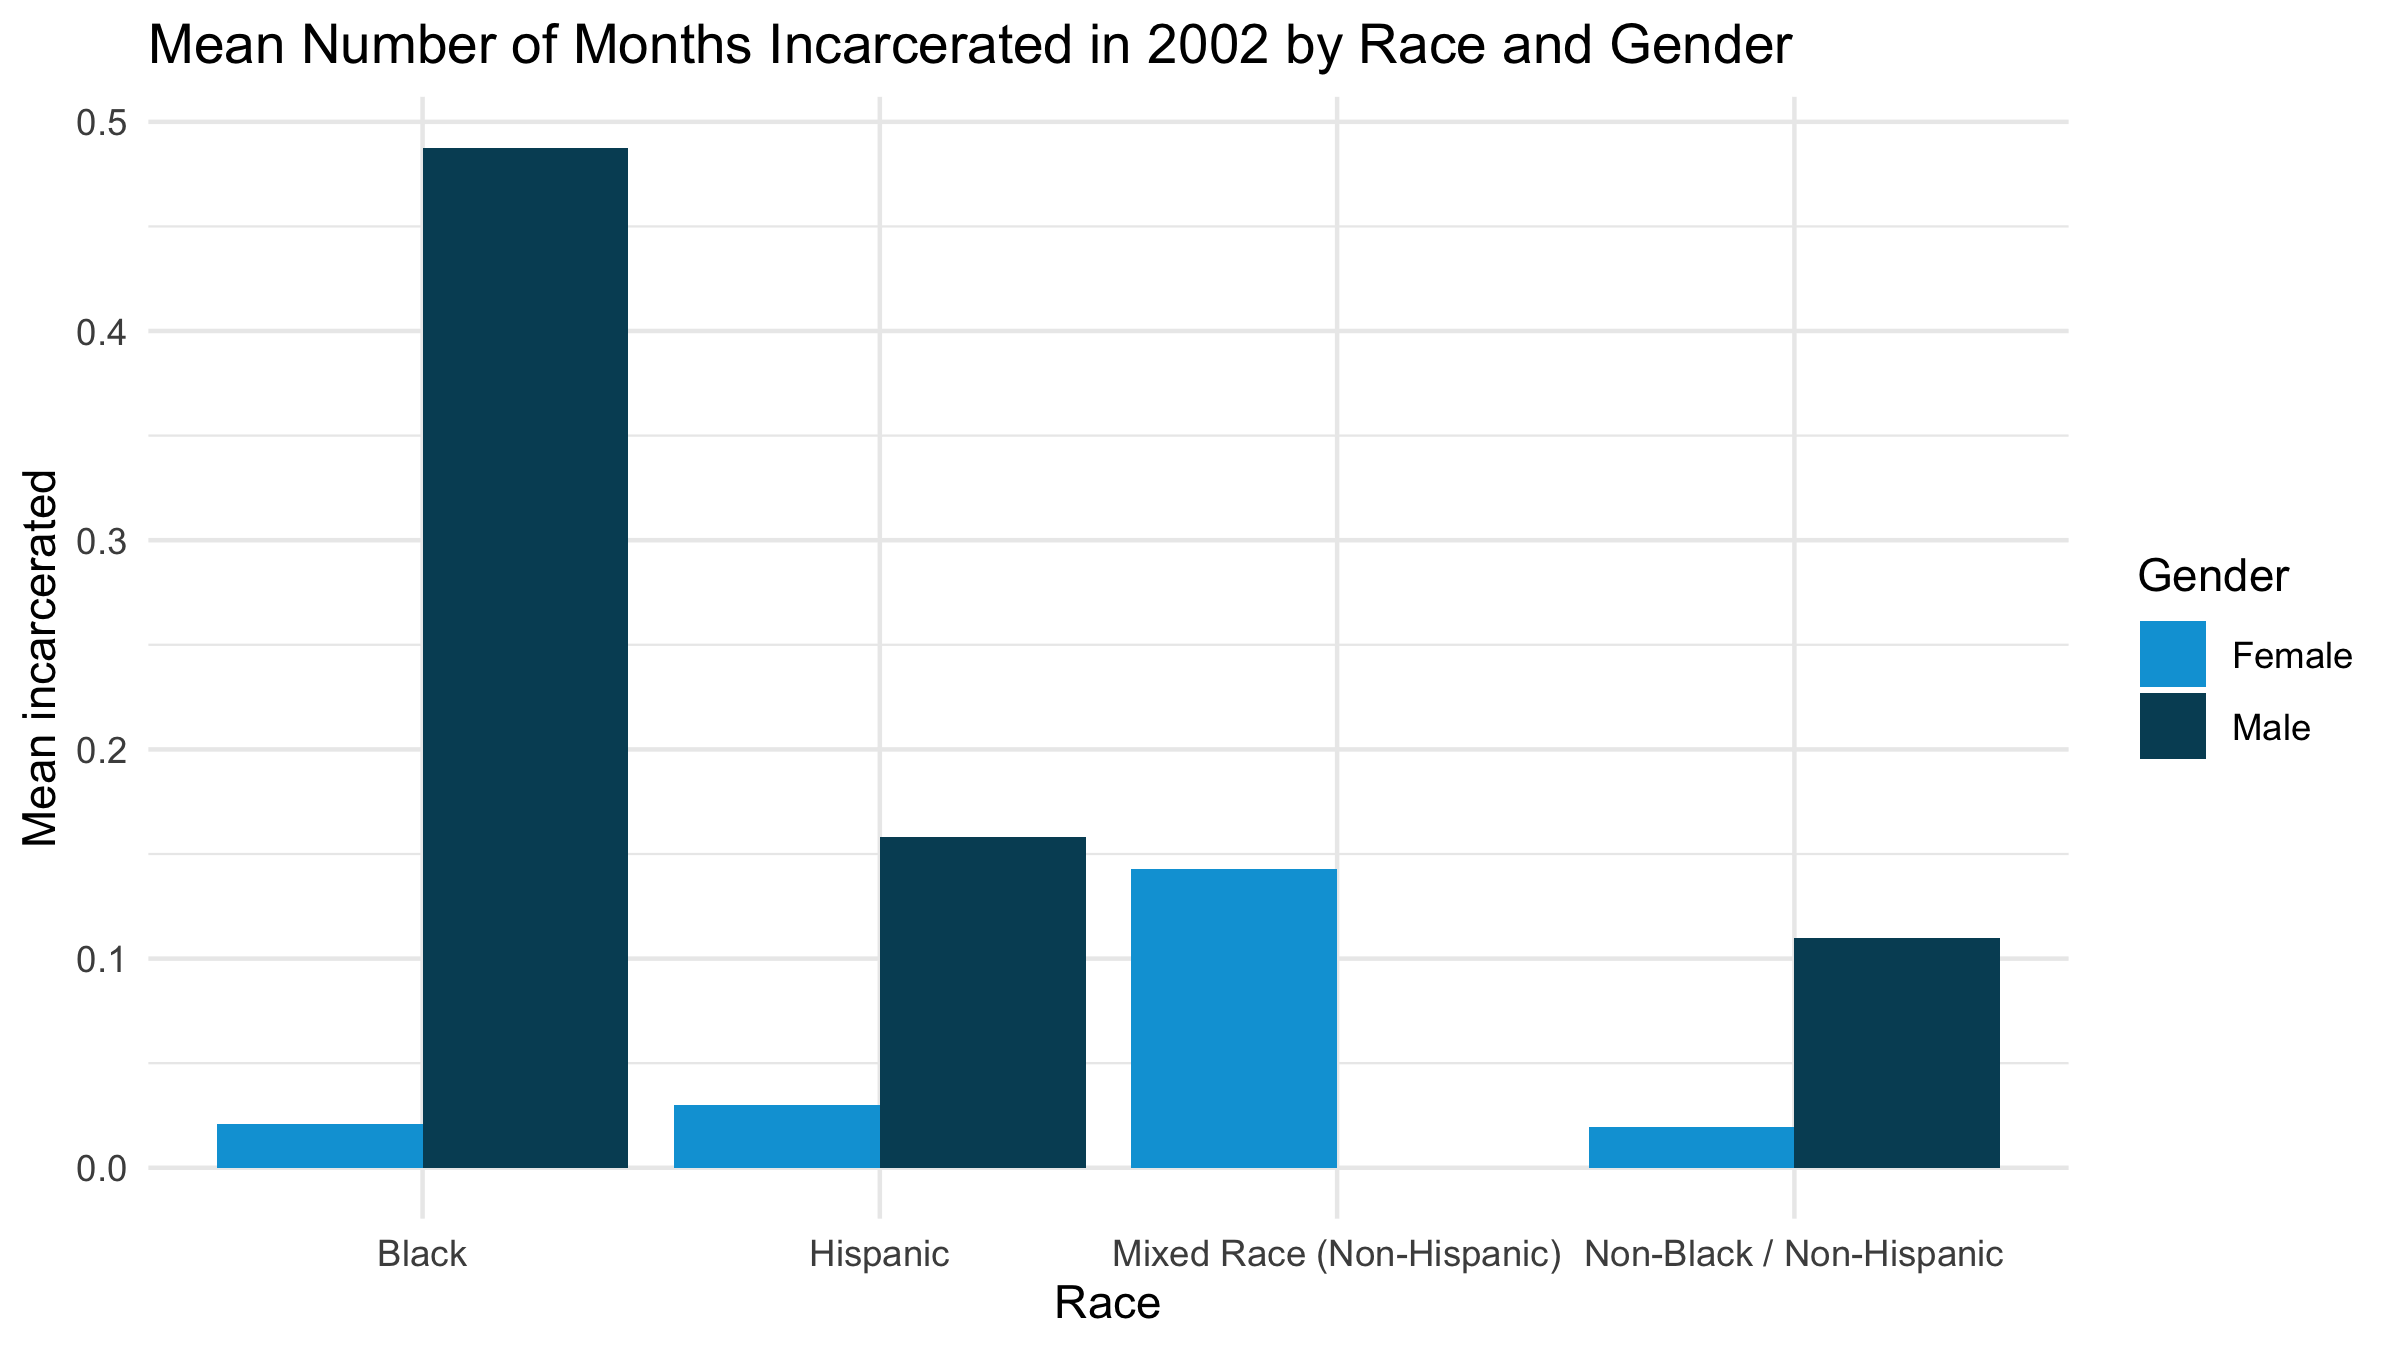
\includegraphics[width=.85\textwidth]{incarcerated_by_racegender}
    \end{center}
    \caption{Mean Number of incarcerated in 2002 by Race and Gender}
    \label{fig:graph}
\end{figure}

We find that across the board, men are more likely to be incarcerated than women. Black men in particular are incarcerated at higher rates than any other race-gender group. A table with the exact values follows.

\begin{table}[H]

\caption{\label{tab:tab:summarystats}Mean Months Incarcerated in 2002 by Race and Gender}
\centering
\begin{tabular}[t]{lrrrr}
\toprule
Gender & Black & Hispanic & Mixed Race Non Hispanic & Non Black Non Hispanic\\
\midrule
\cellcolor{gray!6}{Female} & \cellcolor{gray!6}{0.0211268} & \cellcolor{gray!6}{0.0298013} & \cellcolor{gray!6}{0.1428571} & \cellcolor{gray!6}{0.0193192}\\
Male & 0.4876712 & 0.1579509 & 0.0000000 & 0.1099476\\
\bottomrule
\end{tabular}
\end{table}


We also fit a linear model of the specification:

$$
    incarcerated = race\beta_1 + gender\beta_2 + \varepsilon
$$

The results are as follows:


% Table created by stargazer v.5.2.2 by Marek Hlavac, Harvard University. E-mail: hlavac at fas.harvard.edu
% Date and time: Wed, Feb 16, 2022 - 20:43:19
\begin{table}[!htbp] \centering 
  \caption{Regression Output. Omitted category is Black Females.} 
  \label{tab:regression} 
\begin{tabular}{@{\extracolsep{5pt}}lc} 
\\[-1.8ex]\hline 
\hline \\[-1.8ex] 
 & \multicolumn{1}{c}{\textit{Dependent variable:}} \\ 
\cline{2-2} 
\\[-1.8ex] & months incarcerated in 2002 \\ 
\hline \\[-1.8ex] 
 Hispanic & $-$0.159$^{***}$ \\ 
  & (0.038) \\ 
  & \\ 
 Mixed Race (Non-Hispanic) & $-$0.174$^{**}$ \\ 
  & (0.083) \\ 
  & \\ 
 Non-Black / Non-Hispanic & $-$0.189$^{***}$ \\ 
  & (0.035) \\ 
  & \\ 
 Male & 0.194$^{***}$ \\ 
  & (0.022) \\ 
  & \\ 
 Constant & 0.155$^{***}$ \\ 
  & (0.026) \\ 
  & \\ 
\hline \\[-1.8ex] 
Observations & 8,621 \\ 
R$^{2}$ & 0.015 \\ 
Adjusted R$^{2}$ & 0.014 \\ 
Residual Std. Error & 1.019 (df = 8616) \\ 
F Statistic & 32.033$^{***}$ (df = 4; 8616) \\ 
\hline 
\hline \\[-1.8ex] 
\textit{Note:}  & \multicolumn{1}{r}{$^{*}$p$<$0.1; $^{**}$p$<$0.05; $^{***}$p$<$0.01} \\ 
\end{tabular} 
\end{table} 


The dataset of respondents is restricted to four races: Non-Black / Non-Hispanic, Hispanic, Black, and Mixed Race (Non-Hispanic). It is also restricted to two genders: male and female. The omitted category is Black females, meaning that the constant is accordant to that population and the covariates are relative to that. We find that respondents who are Hispanic or Non-Black / Non-Hispanic tend to have spent 0.159 and 0.189 less months in prison respectively, which is significant at the 0.01 level. We also find that being Mixed Race spent less time incarcerated, which is significant at the 0.05 level.

We find that being male is associated with 0.194 more months spent incarcerated, significant at the 0.01 level.
\end{document}